En este caso, la concentración en la placa es $C_{A_0}$ y lejos de la placa es $C_{A_\infty}\rightarrow0$. LA reacción está dada por $R_A=-k_nC_A^n$. La concentración de A disuelta es pequeña por lo que $\mu, \rho$ y $D_{AB}$ son constantes en el fluido. EL sistema esquematizado en la figura 3.1

\begin{tikzpicture}[scale=3]
\draw[thick] (0,-0.05) rectangle (2.6,0);
\node[below] at (1.3,-0.05) {\large $C_{A0}$};
\draw[very thick] (0,0) .. controls (1.0,1.0) .. (2.4,1.5) node[right] {$\delta(x)$};
\draw[very thick] (0,0) .. controls (1.0,0.4) .. (2.4,0.6) node[right] {$\delta_c(x)$};
\draw[thick] (1.5,0.455) -- (2,0);
\draw[->,thick] (1.67,0.3) -- (1.9,0.3);
\node at (2.3,0.22) {$\dfrac{C_A}{C_{A0}} = 1 - \dfrac{y}{\delta_c}$};
\draw [thick] (1.5,0) -- (1.5,1.5);
\draw [->,thick] (1.5,0.8) -- (1.65,0.8);
\node at (1.9,0.8) {$\dfrac{C_A}{C_{A0}} = 0$};
\draw [thick] (0.5,0) -- (.5,1.5);
\draw[thick](0.5,0)--(0.8,0.6);
\draw[thick](0.8,0.6)--(0.8,1.5);
\node at (0.25,0.4) {\large $\underrightarrow{v_\infty}$};
\foreach \i in {0,1,...,9}
  \draw[->, thick] (0.5,{1.5 - 0.1*\i}) -- (0.8,{1.5 - 0.1*\i});
\draw[->,thick](0.5,0.5)--(0.75,0.5);
\draw[->,thick](0.5,0.4)--(0.7,0.4);
\draw[->,thick](0.5,0.3)--(0.65,0.3);
\draw[->,thick](0.5,0.2)--(0.6,0.2);
\draw[->,thick](0.5,0.1)--(0.55,0.1);
\draw[->, thick] (0.57,0.15) -- (0.8,0.15);
\node[above right] at (0.8,0.03) {$\dfrac{v_x}{{v}_\infty} = \dfrac{y}{\delta}$};
\node[above right] at (0.8,1.3) {$\dfrac{v_x}{{v}_\infty} = 1$};
\draw[->,thick](0.8,1.2)--(0.9,1.3);
\end{tikzpicture}

\label{Fig_3.1}

Fig (3.1) Perfiles de concentración y velocidad para un capa límite laminar con reacción química homogénea 


Las condiciones en la frontera son:
\begin{equation*}
    \frac{v_x}{v_\infty}|_{y\leq\delta (x)}=\frac{y}{\delta}
\end{equation*}
  \begin{equation}
      \frac{v_x}{v_\infty}|_{y\geq\delta (x)}=1
  \end{equation}
\begin{equation*}
    \frac{C_A}{C_{A_0}}|_{y\leq\delta_c(x)}=1-\frac{y}{\delta}
\end{equation*}
\begin{equation}
    \frac{C_A}{C_{A_0}}|_{y\geq\delta_c(x)}=0
\end{equation}
Definiendo $\Delta=\frac{\delta_c}{\delta}$ y suponiendo que $\Delta\leq1$ (La capa límite de concentración se encuentra dentro de la capa límite de velocidad). Además $v_o=v_y|_{y=0}\rightarrow 0$, la ecuación (3.5) se aplica al perfil de $v_x=\frac{v_\infty y}{\delta}$:
\begin{equation*}
    \mu\frac{v_\infty}{\delta}=\frac{d}{dx}\int_0^\infty \rho (v_xv_\infty-v_x^2)dy=\rho v_\infty^2 \frac{d}{dx}\int_0^\infty (\frac{v_x}{v_\infty}-\frac{v_x^2}{v_\infty^2})dy
\end{equation*}
\begin{equation}
    =\frac{d}{dx}[\rho v_\infty^2\int_0^\infty(\frac{y}{\delta}-\frac{y^2}{\delta ^2})dy]=\frac{d}{dx}\rho v_\infty^2 (\frac{y^2}{2\delta}-\frac{y^3}{3\delta ^2})|_0^\infty=\frac{d}{dx}[\rho v_\infty ^2 \delta (\frac{1}{6})]
\end{equation}
 En términos de cantidades molares, la ec (3.7) aplica a al perfil $\frac{C_A}{C_{A_0}}=1-\frac{y}{\delta_c}$   
 \begin{equation*}
     -\frac{D_{AB}C_{A_0}}{\Delta \delta}=\frac{d}{dx}\int_0^\infty v_x(C_{A_\infty}-C_A)dy+\int_0^\infty R_A dy
 \end{equation*}
\begin{equation*}
    =\frac{d}{dx}[\frac{v_\infty}{\delta}\int_0^\infty y(-1+\frac{y}{\delta _c})C_{A_0}dy]=\frac{d}{dx}[\frac{v_\infty C_{A_0}}{\delta}\delta_c^2(\frac{-1}{2}+\frac{1}{3})]
\end{equation*}
\begin{equation*}
    -\frac{D_{AB}C_{A_0}}{\Delta \delta}=\frac{d}{dx}[v_\infty C_{A_0}\delta \Delta^2(-\frac{1}{6})]+k_nC_{A_0}^n \int_0^\infty (1-\frac{y}{\delta_c})^ndy
\end{equation*}
\begin{equation}
    -\frac{D_{AB}C_{A_0}}{\Delta \delta}=\frac{d}{dx}[-\frac{1}{6}v_\infty C_{A_0}\delta \Delta^2]-\frac{k_nC_{A_0}^n}{n+1}\delta \Delta
\end{equation}
La Ec (3.10) se integra: $\frac{6\mu v_\infty}{\rho v_\infty ^2}=\delta\frac{d(\delta)}{dx}$
\begin{equation}
    \delta \frac{d}{dx}(\delta)=\frac{1}{2}\frac{d}{dx}(\delta^2) \rightarrow12\frac{\nu}{v_\infty}(x)=\delta^2
\end{equation}
Multiplicando la ec (3.11) por $-\frac{\Delta \delta}{C_{A_0}\nu}$, se obtiene:
\begin{equation*}
    \frac{D_{AB}}{\nu}=\frac{1}{6}\frac{v_\infty}{\nu}(\Delta \delta)\frac{d}{dx}(\delta \Delta^2)+\frac{k_n}{\nu}(\frac{C_{A_0}^{n-1}}{n+1})\delta^2 \Delta^2
\end{equation*}
Definiendo al número de Schmidt como $Sc=\frac{\nu}{D_{AB}}$, se obtiene:
\begin{equation*}
    \frac{1}{Sc}=\frac{v_\infty}{6\nu}(\Delta \delta)(\Delta^2\frac{d\delta}{dx}+2\Delta \delta \frac{d\Delta}{dx})+\frac{k_n}{\nu}(\frac{C_{A_0}^{n-1}}{n+1})(\frac{12\nu x}{v_\infty})(\Delta^2)
\end{equation*}
Como $\delta \frac{d}{dx}(\delta)=\frac{1}{2}\frac{d(\delta^2)}{dx}=6\frac{\nu}{v_\infty}$ y $\Delta^2\frac{d\Delta}{dx}=\frac{1}{3}\frac{d}{dx}(\Delta^3)$, luego entonces:
\begin{equation*}
    \frac{1}{Sc}=\Delta^3+\frac{v_\infty}{6 \nu}(\frac{12\nu x}{v_\infty})[\frac{2}{3}\frac{d}{dx}\Delta^3)]+12\frac{k_nC_{A_0}^{n-1}}{n+1}(\frac{x}{v_\infty})\Delta^2
\end{equation*}
\begin{equation}
    \frac{1}{Sc}=\Delta^3+\frac{4}{3}x\frac{d}{dx}(\Delta^3)+12\frac{k_nC_{A_0}^{n-1}}{n+1}(\frac{x}{v_\infty})\Delta^2
\end{equation}
Si la reacción no ocurre, entonces $k_n=0$ y la ec (3.15) se reduce a:
\begin{equation}
    \frac{4}{3}x\frac{d}{dx}(\Delta^3)+\Delta^3-\frac{1}{Sc}=0
\end{equation}
Cuya solución es:

\begin{equation*}
    \Delta^3=[c+\int \frac{1}{Sc}(\frac{3}{4x})exp(\int\frac{3}{4x}dx)dx]exp(-\int \frac{3}{4x}dx)
\end{equation*}
Donde c es la constante de integración. Efectuando las operaciones:
\begin{equation*}
    \Delta^3=[c+\frac{3}{4 Sc}\int \frac{1}{x}(x^{\frac{3}{4}})dx]x^{-\frac{3}{4}}
\end{equation*}
\begin{equation*}
    \Delta^3=\frac{c}{x^{3/4}}+\frac{3}{4Sc}x^{\frac{3}{4}}(\frac{4}{3})x^{-\frac{3}{4}}
\end{equation*}
\begin{equation}
    \Delta^3=\frac{c}{x^{\frac{3}{4}}}+\frac{1}{Sc}
\end{equation}
La constante se determina con la condición $\Delta|_{x\rightarrow 0}=finito$, que implica que:
\begin{equation}
    c=0\rightarrow\Delta= Sc^{-\frac{1}{3}}; \forall\Delta<1
\end{equation}
Esta última ecuación a su vez implica que, puesto que $\Delta\equiv\frac{\delta_c}{\delta}$, cuando no hay reacción, el cociente de los grosores de la capa límite de concentración y la capa límite de velocidad es constante. Los límites de reacción lenta y rápida pueden obtenerse a partir de la ecuación (3.13). Para reacción lenta (x pequeño), se propone la siguiente serie:
\begin{equation}
    \Delta= Sc^{-\frac{1}{3}}(1+a_1\xi+...)
\end{equation}
En donde:
\begin{equation}
    \xi=12[k_n\frac{C_{A_0}^{n-1}}{n+1}\frac{x}{v_\infty}]
\end{equation}
Substituyendo la ecuación (3.17) en la ecuación (3.13)
\begin{equation*}
    \frac{1}{Sc}=\frac{1}{Sc}(1+a_1\xi)^3+4x\Delta^2\frac{d\Delta}{dx}+\xi\Delta^2
\end{equation*}
Como $\frac{d\Delta}{dx}=\frac{d}{dx}[Sc^{-\frac{1}{3}}(1+a_1\xi)]=Sc^{-\frac{1}{3}}a_1\frac{d\xi}{dx}$ y si $x\frac{d\xi}{dx}=\xi$
\begin{equation*}
    \frac{1}{Sc}=\frac{1}{Sc}(1+a_1\xi)^3+Sc^{-\frac{2}{3}}(1+a_1\xi)^2[4Sc^{-\frac{1}{3}}a_1\xi+\xi]
\end{equation*}
\begin{equation*}
    \frac{1}{Sc}=\frac{1}{Sc}(1+a_1\xi)^3+\frac{4}{Sc}a_1\xi (1+a_1\xi)^2+\frac{Sc^{\frac{1}{3}}}{Sc}\xi(1+a_1\xi)^2
\end{equation*}
Multiplicando toda la expresión por Sc
\begin{equation*}
    1=(1+a_1\xi)+\xi(1+a_1\xi)^2(4a_1++Sc^{\frac{1}{3}})
\end{equation*}
Linealizando:
\begin{equation*}
    0=3a_1\xi+\xi(4a_1+Sc^{\frac{1}{3}})\rightarrow0=7a_1\xi+\xi Sc^{\frac{1}{3}}
\end{equation*}
Lo que implica que:
\begin{equation}
    a_1=-\frac{Sc^{\frac{1}{3}}}{7}
\end{equation}
Las ecuaciones (3.16) y (3.17) quedan así: 

Sin reacción:
\begin{equation*}
    \Delta =Sc^{-\frac{1}{3}}
\end{equation*}
Con reacción lenta:
\begin{equation}
    \Delta=Sc^{-\frac{1}{3}}(1-\frac{1}{7}Sc^{\frac{1}{3}}\xi)
\end{equation}
Donde $\xi$ está dado por en la ecuación (3.18). La ecuación (3.20) implica que el grosor de la capa límite de concentración disminuye con la reacción química.
Para una reacción rápida, se propone que $\Delta\sim \xi^{-\frac{1}{2}}$, es decir, que $\Delta=c\xi^{-\frac{1}{2}}$ en donde c es una constante. Sustituyendo esta expresión de $\Delta$ en la ecuación (3.13), se tiene:
\begin{equation*}
    \frac{1}{Sc}=\frac{4xc^3}{3}\frac{d}{dx}(\xi^{-\frac{3}{2}})+c^3\xi^{-\frac{3}{2}}+\xi c^2\xi^-1
\end{equation*}
Lo cual implica que el valor dominante de la serie a medida que $\xi$ aumenta corresponde a:
\begin{equation*}
    \frac{1}{Sc}=c^2\rightarrow c=Sc^{-\frac{1}{2}}
\end{equation*}
Y así, para $\xi$ grande:
\begin{equation}
    \Delta=(Sc\xi)^{-\frac{1}{2}}
\end{equation}
La ecuación (3.21) implica que $\frac{\delta_c}{\delta}=\frac{1}{(Sc\xi)^{-\frac{1}{2}}}$, que junto con la ecuación (3.12) revela que:
\begin{equation*}
    \delta_c=\frac{1}{(Sc\xi)^{\frac{1}{2}}}(\frac{12\nu x}{v_\infty})^{\frac{1}{2}}=\sqrt{\frac{12\nu x}{Sc\xi v_\infty}}
\end{equation*}
Cuando x es grande, $\delta_c$ es constante.
